\hypertarget{widgets-1}{%
\section{Widgets (1)}\label{widgets-1}}

\hypertarget{gtklabel-gtkbutton-and-gtkbox}{%
\subsection{GtkLabel, GtkButton and
GtkBox}\label{gtklabel-gtkbutton-and-gtkbox}}

\hypertarget{gtklabel}{%
\subsubsection{GtkLabel}\label{gtklabel}}

In the previous section we made a window and displayed it on the screen.
Now we go on to the next topic, where we add widgets to this window. The
simplest widget is GtkLabel. It is a widget with text in it.

\begin{lstlisting}[language=C, numbers=left]
#include <gtk/gtk.h>

static void
app_activate (GApplication *app, gpointer user_data) {
  GtkWidget *win;
  GtkWidget *lab;

  win = gtk_application_window_new (GTK_APPLICATION (app));
  gtk_window_set_title (GTK_WINDOW (win), "lb1");
  gtk_window_set_default_size (GTK_WINDOW (win), 400, 300);

  lab = gtk_label_new ("Hello.");
  gtk_window_set_child (GTK_WINDOW (win), lab);

  gtk_widget_show (win);
}

int
main (int argc, char **argv) {
  GtkApplication *app;
  int stat;

  app = gtk_application_new ("com.github.ToshioCP.lb1", G_APPLICATION_FLAGS_NONE);
  g_signal_connect (app, "activate", G_CALLBACK (app_activate), NULL);
  stat =g_application_run (G_APPLICATION (app), argc, argv);
  g_object_unref (app);
  return stat;
}
\end{lstlisting}

Save this program to a file \passthrough{\lstinline!lb1.c!}. Then
compile and run it.

\begin{lstlisting}
$ comp lb1
$ ./a.out
\end{lstlisting}

A window with a message ``Hello.'' appears.

\begin{figure}
\centering
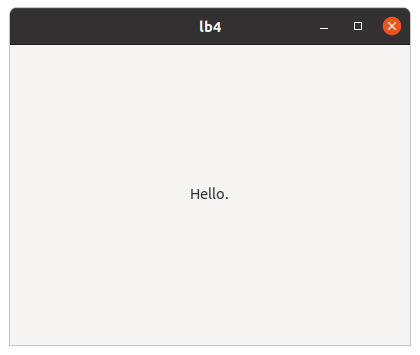
\includegraphics[width=6.3cm,height=5.325cm]{../image/screenshot_lb1.png}
\caption{Screenshot of the label}
\end{figure}

There's only a little change between \passthrough{\lstinline!pr4.c!} and
\passthrough{\lstinline!lb1.c!}. A program
\passthrough{\lstinline!diff!} is good to know the difference between
two files.

\begin{lstlisting}
$ cd misc; diff pr4.c lb1.c
5a6
>   GtkWidget *lab;
8c9
<   gtk_window_set_title (GTK_WINDOW (win), "pr4");
---
>   gtk_window_set_title (GTK_WINDOW (win), "lb1");
9a11,14
> 
>   lab = gtk_label_new ("Hello.");
>   gtk_window_set_child (GTK_WINDOW (win), lab);
> 
18c23
<   app = gtk_application_new ("com.github.ToshioCP.pr4", G_APPLICATION_FLAGS_NONE);
---
>   app = gtk_application_new ("com.github.ToshioCP.lb1", G_APPLICATION_FLAGS_NONE);
\end{lstlisting}

This tells us:

\begin{itemize}
\tightlist
\item
  The definition of a new variable \passthrough{\lstinline!lab!} is
  added.
\item
  The title of the window is changed.
\item
  A label is created and connected to the window as a child.
\end{itemize}

The function
\passthrough{\lstinline!gtk\_window\_set\_child (GTK\_WINDOW (win), lab)!}
makes the label \passthrough{\lstinline!lab!} a child widget of the
window \passthrough{\lstinline!win!}. Be careful. A child widget is
different from a child object. Objects have parent-child relationships
and widgets also have parent-child relationships. But these two
relationships are totally different. Don't be confused. In the program
\passthrough{\lstinline!lb1.c!}, \passthrough{\lstinline!lab!} is a
child widget of \passthrough{\lstinline!win!}. Child widgets are always
located in their parent widget on the screen. See how the window has
appeared on the screen. The application window includes the label.

The window \passthrough{\lstinline!win!} doesn't have any parents. We
call such a window top-level window. An application can have more than
one top-level window.

\hypertarget{gtkbutton}{%
\subsubsection{GtkButton}\label{gtkbutton}}

The next widget to introduce is GtkButton. It displays a button on the
screen with a label or icon on it. In this subsection, we will make a
button with a label. When the button is clicked, it emits a ``clicked''
signal. The following program shows how to catch the signal to then do
something.

\begin{lstlisting}[language=C, numbers=left]
#include <gtk/gtk.h>

static void
click_cb (GtkButton *btn, gpointer user_data) {
  g_print ("Clicked.\n");
}

static void
app_activate (GApplication *app, gpointer user_data) {
  GtkWidget *win;
  GtkWidget *btn;

  win = gtk_application_window_new (GTK_APPLICATION (app));
  gtk_window_set_title (GTK_WINDOW (win), "lb2");
  gtk_window_set_default_size (GTK_WINDOW (win), 400, 300);

  btn = gtk_button_new_with_label ("Click me");
  gtk_window_set_child (GTK_WINDOW (win), btn);
  g_signal_connect (btn, "clicked", G_CALLBACK (click_cb), NULL);

  gtk_widget_show (win);
}

int
main (int argc, char **argv) {
  GtkApplication *app;
  int stat;

  app = gtk_application_new ("com.github.ToshioCP.lb2", G_APPLICATION_FLAGS_NONE);
  g_signal_connect (app, "activate", G_CALLBACK (app_activate), NULL);
  stat =g_application_run (G_APPLICATION (app), argc, argv);
  g_object_unref (app);
  return stat;
}
\end{lstlisting}

Look at the line 17 to 19. First, it creates a GtkButton instance
\passthrough{\lstinline!btn!} with a label ``Click me''. Then, adds the
button to the window \passthrough{\lstinline!win!} as a child. Finally,
connects a ``clicked'' signal of the button to a handler (function)
\passthrough{\lstinline!click\_cb!}. So, if
\passthrough{\lstinline!btn!} is clicked, the function
\passthrough{\lstinline!click\_cb!} is invoked. The suffix ``cb'' means
``call back''.

Name the program \passthrough{\lstinline!lb2.c!} and save it. Now
compile and run it.

\begin{figure}
\centering
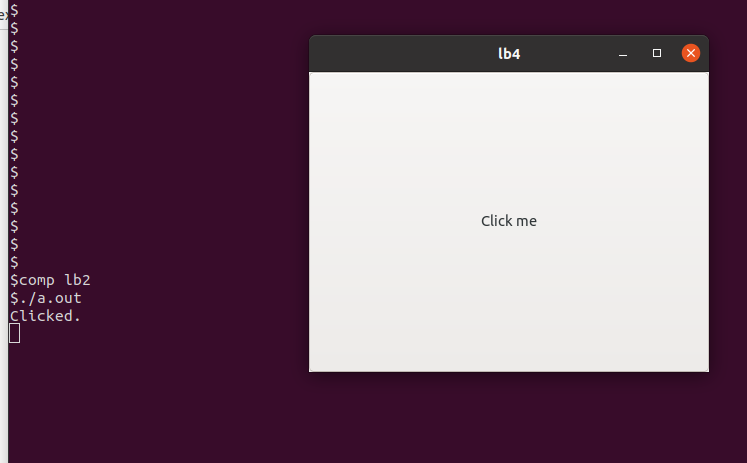
\includegraphics[width=11.205cm,height=6.945cm]{../image/screenshot_lb2.png}
\caption{Screenshot of the label}
\end{figure}

A window with the button appears. Click the button (it is a large
button, you can click everywhere in the window), then a string
``Clicked.'' appears on the terminal. It shows the handler was invoked
by clicking the button.

It's good that we make sure that the clicked signal was caught and the
handler was invoked by using \passthrough{\lstinline!g\_print!}.
However, using g\_print is out of harmony with Gtk which is a GUI
library. So, we will change the handler. The following code is
\passthrough{\lstinline!lb3.c!}.

\begin{lstlisting}[language=C, numbers=left]
static void
click_cb (GtkButton *btn, gpointer user_data) {
  GtkWindow *win = GTK_WINDOW (user_data);
  gtk_window_destroy (win);
}

static void
app_activate (GApplication *app, gpointer user_data) {
  GtkWidget *win;
  GtkWidget *btn;

  win = gtk_application_window_new (GTK_APPLICATION (app));
  gtk_window_set_title (GTK_WINDOW (win), "lb3");
  gtk_window_set_default_size (GTK_WINDOW (win), 400, 300);

  btn = gtk_button_new_with_label ("Quit");
  gtk_window_set_child (GTK_WINDOW (win), btn);
  g_signal_connect (btn, "clicked", G_CALLBACK (click_cb), win);

  gtk_widget_show (win);
}
\end{lstlisting}

And the difference between \passthrough{\lstinline!lb2.c!} and
\passthrough{\lstinline!lb3.c!} is as follows.

\begin{lstlisting}
$ cd misc; diff lb2.c lb3.c
5c5,6
<   g_print ("Clicked.\n");
---
>   GtkWindow *win = GTK_WINDOW (user_data);
>   gtk_window_destroy (win);
14c15
<   gtk_window_set_title (GTK_WINDOW (win), "lb2");
---
>   gtk_window_set_title (GTK_WINDOW (win), "lb3");
17c18
<   btn = gtk_button_new_with_label ("Click me");
---
>   btn = gtk_button_new_with_label ("Quit");
19c20
<   g_signal_connect (btn, "clicked", G_CALLBACK (click_cb), NULL);
---
>   g_signal_connect (btn, "clicked", G_CALLBACK (click_cb), win);
29c30
<   app = gtk_application_new ("com.github.ToshioCP.lb2", G_APPLICATION_FLAGS_NONE);
---
>   app = gtk_application_new ("com.github.ToshioCP.lb3", G_APPLICATION_FLAGS_NONE);
35d35
< 
\end{lstlisting}

The changes are:

\begin{itemize}
\tightlist
\item
  The function \passthrough{\lstinline!g\_print!} in
  \passthrough{\lstinline!lb2.c!} was deleted and the two lines above
  are inserted instead.
\item
  The label of \passthrough{\lstinline!btn!} is changed from ``Click
  me'' to ``Quit''.
\item
  The fourth argument of \passthrough{\lstinline!g\_signal\_connect!} is
  changed from \passthrough{\lstinline!NULL!} to
  \passthrough{\lstinline!win!}.
\end{itemize}

The most important change is the fourth argument of
\passthrough{\lstinline!g\_signal\_connect!}. This argument is described
as ``data to pass to handler'' in the definition of
\passthrough{\lstinline!g\_signal\_connect!} in
\href{https://docs.gtk.org/gobject/func.signal_connect.html}{GObject API
Reference}. Therefore, \passthrough{\lstinline!win!} which is a pointer
to GtkApplicationWindow is passed to the handler as a second parameter
\passthrough{\lstinline!user\_data!}. The handler then casts it to a
pointer to GtkWindow and calls
\passthrough{\lstinline!gtk\_window\_destroy!} to destroy the top-level
window. The application then quits.

\hypertarget{gtkbox}{%
\subsubsection{GtkBox}\label{gtkbox}}

GtkWindow and GtkApplicationWindow can have only one child. If you want
to add two or more widgets in a window, you need a container widget.
GtkBox is one of the containers. It arranges two or more child widgets
into a single row or column. The following procedure shows the way to
add two buttons in a window.

\begin{itemize}
\tightlist
\item
  Create a GtkApplicationWindow instance.
\item
  Create a GtkBox instance and add it to the GtkApplicationWindow as a
  child.
\item
  Create a GtkButton instance and append it to the GtkBox.
\item
  Create another GtkButton instance and append it to the GtkBox.
\end{itemize}

After this, the Widgets are connected as the following diagram.

\begin{figure}
\centering
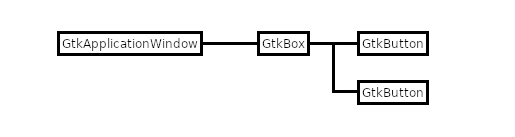
\includegraphics[width=7.725cm,height=2.055cm]{../image/box.png}
\caption{Parent-child relationship}
\end{figure}

The program \passthrough{\lstinline!lb4.c!} includes these widgets. It
is as follows.

\begin{lstlisting}[language=C, numbers=left]
#include <gtk/gtk.h>

static void
click1_cb (GtkButton *btn, gpointer user_data) {
  const gchar *s;

  s = gtk_button_get_label (btn);
  if (g_strcmp0 (s, "Hello.") == 0)
    gtk_button_set_label (btn, "Good-bye.");
  else
    gtk_button_set_label (btn, "Hello.");
}

static void
click2_cb (GtkButton *btn, gpointer user_data) {
  GtkWindow *win = GTK_WINDOW (user_data);
  gtk_window_destroy (win);
}

static void
app_activate (GApplication *app, gpointer user_data) {
  GtkWidget *win;
  GtkWidget *box;
  GtkWidget *btn1;
  GtkWidget *btn2;

  win = gtk_application_window_new (GTK_APPLICATION (app));
  gtk_window_set_title (GTK_WINDOW (win), "lb4");
  gtk_window_set_default_size (GTK_WINDOW (win), 400, 300);

  box = gtk_box_new (GTK_ORIENTATION_VERTICAL, 5);
  gtk_box_set_homogeneous (GTK_BOX (box), TRUE);
  gtk_window_set_child (GTK_WINDOW (win), box);

  btn1 = gtk_button_new_with_label ("Hello.");
  g_signal_connect (btn1, "clicked", G_CALLBACK (click1_cb), NULL);

  btn2 = gtk_button_new_with_label ("Quit");
  g_signal_connect (btn2, "clicked", G_CALLBACK (click2_cb), win);

  gtk_box_append (GTK_BOX (box), btn1);
  gtk_box_append (GTK_BOX (box), btn2);

  gtk_widget_show (win);
}

int
main (int argc, char **argv) {
  GtkApplication *app;
  int stat;

  app = gtk_application_new ("com.github.ToshioCP.lb4", G_APPLICATION_FLAGS_NONE);
  g_signal_connect (app, "activate", G_CALLBACK (app_activate), NULL);
  stat =g_application_run (G_APPLICATION (app), argc, argv);
  g_object_unref (app);
  return stat;
}
\end{lstlisting}

Look at the function \passthrough{\lstinline!app\_activate!}.

After the creation of a GtkApplicationWindow instance, a GtkBox instance
is created.

\begin{lstlisting}
box = gtk_box_new(GTK_ORIENTATION_VERTICAL, 5);
gtk_box_set_homogeneous (GTK_BOX (box), TRUE);
\end{lstlisting}

The first argument arranges the children of the box vertically. The
second argument is the size between the children. The next function
fills the box with the children, giving them the same space.

After that, two buttons \passthrough{\lstinline!btn1!} and
\passthrough{\lstinline!btn2!} are created and the signal handlers are
set. Then, these two buttons are appended to the box.

\begin{figure}
\centering
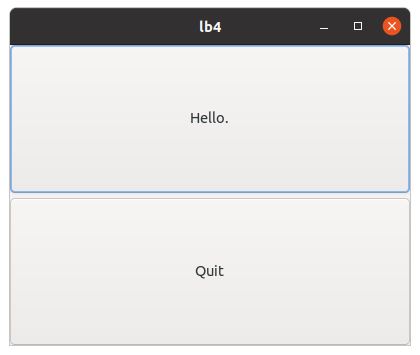
\includegraphics[width=6.3cm,height=5.325cm]{../image/screenshot_lb4.png}
\caption{Screenshot of the box}
\end{figure}

The handler corresponds to \passthrough{\lstinline!btn1!} toggles its
label. The handler corresponds to \passthrough{\lstinline!btn2!}
destroys the top-level window and the application quits.
